%Präambel
\documentclass[paper=a4,fontsize=11pt,headsepline,footsepline,parskip=half]{scrartcl}
\usepackage[utf8]{inputenc}
\usepackage[T1]{fontenc}
\usepackage{amsmath,amsfonts,amssymb}
\usepackage{ngerman,graphicx,textcomp,mathpazo,booktabs}
\usepackage[decimalsymbol=comma,per=frac]{siunitx}
\usepackage[textfont=sl,labelfont=bf]{caption}[2013/05/02]

%Seite einrichten
\areaset[2cm]		% Zusätzlicher Rand für die Bindung
        {17cm}{24cm}	% Textbreite und -Höhe

%Zeilenabstand
\linespread{1.2} %Standardwert

%Linienstärke
\newcommand\HRule{\noindent\rule{\linewidth}{1.5pt}}

%Kopf- und Fußzeile
\usepackage{scrlayer-scrpage}
\setlength{\headheight}{23pt}
\lohead{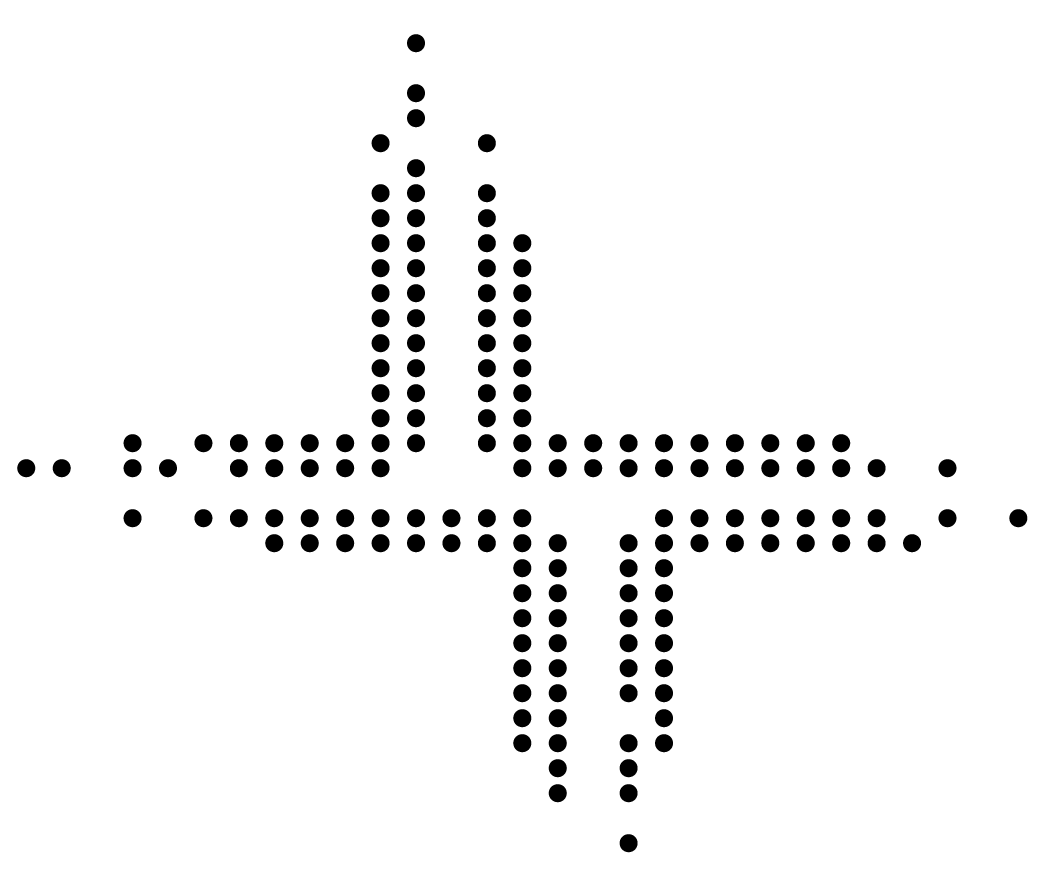
\includegraphics[width=0.7cm]{logofbi} Hochschule Darmstadt}
\rohead{David Falk, Christian Lichtsinn}
\pagestyle{scrheadings}

%sollte als letztes Paket geladen werden
\usepackage{hyperref}

\begin{document}

%Titelblatt
\begin{titlepage}

\begin{minipage}[c]{5cm}
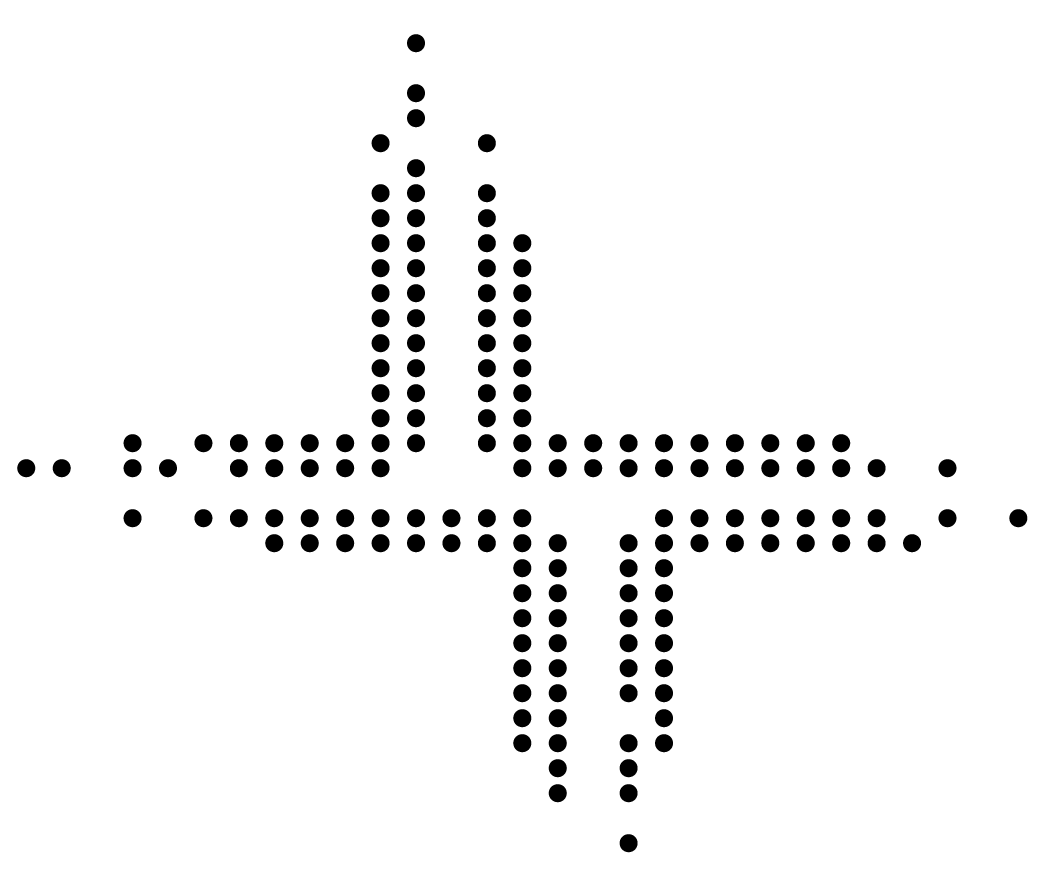
\includegraphics[width=5cm]{logofbi}
\end{minipage}
\hfill
\begin{minipage}[c]{10cm}
\begin{flushright}
\Large Einführung in die Technik\\und Anwendung von\\
\LARGE \textbf{RFID}
\end{flushright}
\end{minipage}

\vspace*{1cm}

\begin{minipage}[c]{8cm}
\begin{flushleft}
\large David Falk (736532)\\Christian Lichtsinn (736787)\\Praktikum 1 \& 2: 19.10.15 \& 02.11.15
\end{flushleft}
\end{minipage}
\hfill
\begin{minipage}[c]{8cm}
\begin{flushright}
\large Betreuer:\\Prof. Ralf S. Mayer\\F. Dotzauer, E. Wagner
\end{flushright}
\end{minipage}

\vspace*{1cm}

\HRule

\vspace*{1cm}

\noindent
\large{Thema: \textbf{AutoID -- Resonanz -- Frequenzen -- RFID-Grundlagen}}

\section{OCR}

Optical character recognition (OCR), bzw. Texterkennung ist eine Methode, mit der man mittels optischer
Eingabegeräte wie Scanner, Kamera oder auch Fax-Gerät Text auf Bildern erkennen und diesen dann auch
digital verarbeiten kann, sofern es denn einwandfrei funktioniert. Dass dem nicht immer so ist zeigt
unter anderem ein Beispielbild auf Wikipedia\footnote{\url{https://de.wikipedia.org/wiki/Texterkennung\#/media/File:Beispiel_Texterkennung.png}}
und ein Vortrag vom 31. Chaos Communication Congress, bei dem Informatiker David Kriesel über die Texterkennung
von Xerox-Scannern berichtet.\footnote{Traue keinem Scan, den du nicht selbst gefälscht hast [31c3] von David Kriesel:\\ \url{https://www.youtube.com/watch?v=Vp03vyNspyI}}

Leider konnten wir aufgrund von fehlender Hardware keine Versuche zu Hause durchführen.

\end{titlepage}

\section{Barcodes}

Barcodes sind parallel nebeneinander aufgestellte Striche verschiedener Dicke, die einen binären Code darstellen,
welcher mit Barcodelesegeräten ausgelesen werden kann. Angewendet werden diese Barcodes vor allem im Einzelhandel und Versand.

\subsection{Welche Arten von Barcodes kann das Gerät erfassen?}

Wir waren in der Lage, folgende Barcodes zu scannen: EAN-8, EAN-13, ISBN (was als EAN-13 ausgegeben wurde),
UPC-A, UPC-E, 3 of 9, Code39, Code128, Code EAN128 sowie Barcodes von Flaschen und den PCs im Labor, welche als EAN-8/13 und Code39 erkannt wurden.

Zusätzlich gab es noch weitere Barcodes, die kurze Texte codiert hatten. Bei einigen stand bereits daneben, welcher Text sich hinter den Barcodes
versteckt (die wir auch bestätigen konnten), bei anderen wurde es nicht verraten. Diese 5 Barcodes enthielten die Texte:
\glqq esaip Angers\grqq{}, \glqq IRT2\grqq{}, \glqq IRT3 \grqq{}, \glqq enjoy the RFID lessons\grqq{} und \glqq good luck for all your studies\grqq{}.

\subsection{Wie viele Barcodes können in einer bestimmten Zeit erfasst werden?}

Die Erfassung durch das Gerät geschieht unverzüglich. Da man das Gerät aber mit der Hand bedienen muss und den
Scanbereich zum Barcode führen muss, kann man ca. 1 Barcode pro Sekunde erfassen.

\subsection{Wie ändert sich die Erkennung mit Abstand, Winkel, Abdeckung, Einfluss von Licht?}

Der Barcode ließ sich geschätzt mit bis zu einem $\SI{0.5}{\meter}$ Abstand vom Lesegerät erfassen. Bis zu einem geschätzten
Winkel von $80\degree$ war der Barcode noch lesbar, solange alle Striche erfasst wurden. War der Barcode abgedeckt, war
für das Lesegerät keine Erkennung mehr möglich. Den Einfluss von Licht konnten wir nicht testen, da wir keine
sehr helle Lichtquelle zur Verfügung hatten, auch nicht das Sonnenlicht, da es am Versuchstag bewölkt war.

\subsection{Welche Auswirkung hätte Verschmutzung, Beschädigung des Barcodes?}

Da das Scannen von Barcodes eine optische Methode ist, ist jede optische Änderung des Barcodes, eben Verschmutzung oder Beschädigung des
Codes ein Problem, das zu Schwierigkeiten oder zum Nicht-Erfassen des Barcodes durch das Lesegerät führt.

\subsection{Hängt die Lesegeschwindigkeit mit der Informationsmenge im Code zusammen?}

Die Erfassung des Codes erfolgt komplett und unverzüglich. Man kann auch nicht sehr viel Information in den Barcodes
speichern und es gab keinen erkennbaren Unterschied bei den Scans. Daher nein.

\section{Oszilloskop, Spektrumanalysator und Frequenzgenerator}

Im Oszilloskop wird die Amplitude gegen die Zeit aufgetragen und das empfangene Signal als Sinuskurve dargestellt. Damit lässt sich u.a.
die Amplitudenmodulation sehr gut darstellen. Dagegen sieht man Seitenbänder kaum. Dafür ist der Spektrumanalysator besser geeignet, bei
dem die Amplitude gegen die Frequenz aufgetragen ist. Damit lassen sich, wie bereits geschrieben, Seitenbänder und damit die Bandbreite
besser darstellen und damit auch besser untersuchen. So sind im Spektrumanalysator z. B. die verschiedenen WLAN-Kanäle deutlich zu erkennen.

\section{Schwingkreis, Resonanz, Lastmodulation und Demodulation}

Bei der Kopplung zweier Schwingkreise, bei dem einer an einen Frequenzgenerator angeschlossen ist und der andere an eine Platine mit
LED kann man die Energieübertragung durch magnetische Kopplung nachweisen. Dabei strahlt die LED heller, je näher man an die
Resonanzfrequenz des Schwingkreises kommt. Hinzukommt die Position der Spulen zueinander. Optimal ist zum einen, wenn die Spulen parallel
zueinander angeordnet sind und dabei einen gewissen Abstand nicht überschreiten (die Strecke, bei der die Magnetfeldlinien der Spule
noch gerade verlaufen). Danach wird die Energieübertragung schwächer. Die Spulen können auch nebeneinander angeordnet werden.

Was hingegen nicht funktioniert ist, wenn die Spulen um $90\degree$ zueinander gedreht sind oder sich unter einer Spule eine Alufolie
befindet, die das Magnetfeld stört.

Um die Resonanzbreite zu bestimmen, muss zuerst die Resonanzkurve gemessen werden. Die Messwerte dazu befinden sich in Tabelle \ref{tab:resonanzkurve}
auf Seite \pageref{tab:resonanzkurve}.

\begin{table}[ht]
\caption{\label{tab:resonanzkurve}Messwerte zur Bestimmung der Resonanzkurve.}
\centering
\begin{tabular}{@{}cccccc@{}}
\toprule
  f [kHz] & U [V] & f [kHz] & U [V] & f [kHz] & U [V]\\
\midrule
 100 & 8,4 & 129 & 61,2 & 139 & 52,4\\
 102 & 9,2 & 130 & 65,2 & 140 & 49,6\\
 110 & 12,8 & 131 & 68,0 & 142 & 44,4\\
 117 & 19,6 & 132 & 68,8 & 144 & 39,2\\
 120 & 24,0 & 133 & 68,0 & 146 & 36,0\\
 122 & 28,8 & 134 & 66,8 & 150 & 30,0\\
 124 & 34,4 & 135 & 64,4 & 155 & 24,4\\
 126 & 43,2 & 136 & 61,2 & 160 & 21,2\\
 127 & 49,2 & 137 & 58,4 & 170 & 17,2\\
 128 & 55,2 & 138 & 55,2 & & \\
\bottomrule
\end{tabular}
\end{table}
\begin{center}
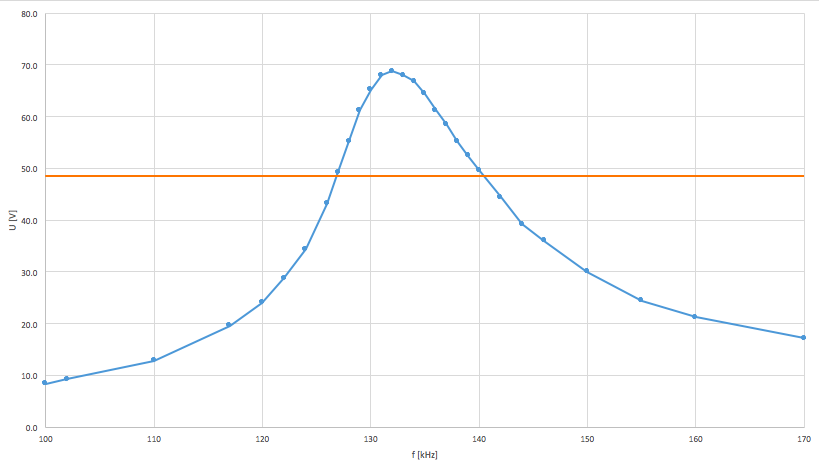
\includegraphics[width=\linewidth]{resonanzkurve.png}
\end{center}

\section{1,3 GHz Mikrowellen}

\subsection{Lineare Polarisation}

Im Gegensatz zur zirkulären Polarisation schwingen die Wellen(?) nur in einer Ebene, zum Beispiel nur senkrecht oder nur waagrecht.
Das hat zur Folge, dass wenn das Lesegerät nicht genauso wie der Sender ausgerichtet ist, das Signal mit jedem Grad Änderung
zur Ausrichtung des Senders schwächer wird, bis es bei $90\degree$ Drehung nicht mehr zu empfangen ist.

\subsection{Absorption}

Je höher die Frequenz ist, desto mehr wird in Flüssigkeiten wie Wasser absorbiert. Das ist für LF noch kein Problem, für Mikrowellen aber schon.
Deswegen sind es vor allem Behälter mit Flüssigkeiten, wie Flaschen oder Menschen, die das Signal erheblich stören. Aber auch
Objekte, die ungefähr so groß wie die Sender-/Empfänger-Antennen sind oder das in Bleistiften enthaltene Graphit haben Einfluss auf das
empfangene Signal. Auch Alufolie ist in der Lage das Signal zu stören, bzw. komplett zu eliminieren.

Dies macht RFID als Labels für Gegenstände mit Flüssigkeiten bzw. aus Metall ungeeignet.

\subsection{Signalstärke zu Abstand}

Die Signalstärke nimmt mit zunehmendem Abstand ab. Es gilt ungefähr
$$\sigma = \frac{1}{r^4}$$

\section{RFID HF}

\section{NFC}

\subsection{Was ist NFC?}

NFC ist RFID, bei der die stikte Trennung zwischen Lesegerät und Tag/Transponder aufgehoben wird.
NFC verwendet den HF-Bereich bei 13,56 MHz.

\subsection{Vorbereitete Tags}

\subsection{Tag konfigurieren}

\subsection{Übertragung zwischen zwei Smartphones}

Mit Android Beam ist es möglich Inhalte zwischen zwei Android-Telefonen übertragen.
Wir konnten eine URL übertragen, wenn eine Website geöffnet ist und den App Store
öffnen, wenn eine App geöffnet ist.

\end{document}
